\chapter{Tips} \label{chapter:tips}

\graphicspath{{Manuscript/Tips/Figs/}}

%=========================================================================
\section{English Writing}

% --------------------------
\subsection{Useful Sites}

\subsubsection{Springer Exemplar}
\url{http://www.springerexemplar.com/}

\subsubsection{Oxford Learner's Dictionaries}
\url{http://www.oxfordlearnersdictionaries.com}

\subsubsection{Thesaurus.com}
\url{http://www.thesaurus.com}


\subsection{Useful Books}

\begin{itemize}
	\item The Elements of Style, Fourth Edition~\cite{strunk1979}
\end{itemize}

%=========================================================================
\section{\LaTeX ~Tips}

% --------------------------
\subsection{Table} \label{sec:table}

Table~\ref{table:running_time} shows a sample.

\begin{table}[tbp]
% h:here, t:top, b:bottom, p:page of floats
\begin{center}
\begin{tabular}{c|ccc}
$n$  & Algorithm A  & Algorithm B & Ours  \\ \hline
20   & 100          & 150         & 10    \\
40   & 200          & 300         & 20    \\
60   & 400          & 600         & 30    \\
\end{tabular}
\caption{Running time}
\label{table:running_time}
\end{center}
\end{table}

% --------------------------
\subsection{Figure}

Figure~\ref{fig:graph} shows a sample.

\begin{figure}[tbp]
% h:here, t:top, b:bottom, p:page of floats
\begin{center} 
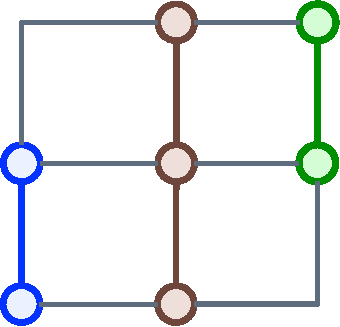
\includegraphics[width=3.5cm]{sample_graph.pdf}
\caption{Input graph}
\label{fig:graph}
\end{center} 
\end{figure}

% --------------------------
\subsection{Algorithm}

A sample from the manual of the algorithmicx package is shown in Algorithm~\ref{alg:euclid}.

\begin{algorithm}
\caption{Euclid's algorithm}\label{alg:euclid}
\begin{algorithmic}[1]
\Procedure{Euclid}{$a,b$}\Comment{The g.c.d. of $a$ and $b$}
   \State $r\gets a\bmod b$
   \While{$r\not=0$}\Comment{We have the answer if $r$ is 0}
      \State $a\gets b$
      \State $b\gets r$
      \State $r\gets a\bmod b$
   \EndWhile\label{euclidendwhile}
   \State \textbf{return} $b$\Comment{The gcd is $b$}
\EndProcedure
\end{algorithmic}
\end{algorithm}

\mytodo[inline]{Write more tips.}



